\vspace{-1em}
\section{The Internet}

\noindent
Terminology and concepts of the internet, which will be used throughout this text.

\begin{Def}[Protocol]

    A \textbf{protocol} is a set of rules which govern the exchange of data between devices. 
    Protocols define the format, timing, sequencing, and error control of data transmission \cite{rfc791}.
\end{Def}

\begin{Def}[Internet]

    The \textbf{Internet} is a global network of distributed system communicating over an \textbf{Internet Protocol} (IP) \cite{cloudflare_internet_protocol}.
    Documents served over the internet are referred to as \textbf{webpages} or \textbf{websites}.
\end{Def}
\begin{Def}[HTTP \& HTML]

    \textbf{HTTP} (HyperText Transfer Protocol), the protocol which transfer data over the internet, 
    distributing \textbf{HTML} (HyperText Markup Language) documents. Such 
    documents include \textbf{hyperlinks} to other websites, images, and other media \cite{rfc9110}.
\end{Def}
\begin{Def}[RFC (Request for Comments)]

    \textbf{RFC} (Request for Comments) is a publication from the \textbf{Internet Engineering Task Force} (IETF) 
    and the \textbf{Internet Society} (ISOC). This body governs the specifications for the internet and its protocols \cite{rfc}.
\end{Def}

\begin{Def}[DNS and IP Addresses]

    An \textbf{Internet Protocol address} (IP address) is a unique identifier for a device on a network. 
    The \textbf{Domain Name System} (DNS) maps domain names to IP addresses \cite{rfc760}.
\end{Def}

\newpage

\begin{Def}[Web Browser]

    A \textbf{web browser} is a software application for accessing the \textbf{World Wide Web} (WWW) \cite{ou_internet_history}.
\end{Def}

\begin{Def}[URL (Uniform Resource Locator)]

    A \textbf{URL} (Uniform Resource Locator) references each webpage, specifying protocol, domain, and path \cite{w3c_html_href_draft}.
    E.g., \texttt{http://www.example.com/path/to/resource}.
    \begin{itemize}
        \item \textbf{Protocol}: \texttt{http}
        \item \textbf{Domain}: \texttt{www.example.com}
        \item \textbf{Path}: \texttt{/path/to/resource}
    \end{itemize}
\end{Def}
\begin{Def}[Client-Server Model]

    Most of the internet operates on a \textbf{client-server model}, where an agent device\textendash the \textbf{client}\textendash requests data from another agent\textendash the \textbf{server}\textendash 
    which serves an appropriate response. Clients are not servers and vice versa, as they receive and interpret data differently \cite{cloudflare_client_server}.
\end{Def}

\begin{Def}[HTTP Methods]
    
        When a client makes a request to a server, they must specify their intent, categorized by \textbf{HTTP methods} \cite{rfc2616}:
        \begin{itemize}
            \item \textbf{GET}: Retrieve data from the server.
            \item \textbf{POST}: Send data to the server.
            \item \textbf{PUT}: Update data on the server.
            \item \textbf{DELETE}: Remove data from the server.
        \end{itemize}
\end{Def}
\begin{Def}[HTTP Headers]

    \textbf{HTTP headers} are key-value pairs sent between the client and server to provide \textbf{metadata} about the request or response.
    \textbf{Metadata} is data about the transmitted data, telling the receiver how the incoming data should be interpreted \cite{rfc2616}.
\end{Def}


\newpage
\noindent
Tim Berners-Lee and his team at CERN developed the first web server and browser in 1989 \cite{w3c_http_history}.

\begin{table}[h!]
    \centering
    \begin{tabular}{@{}p{3cm}p{10cm}@{}}
    \toprule
    \textbf{HTTP Version} & \textbf{Description} \\ \midrule
    HTTP/0.9 (1991)       & Only supports GET method (retrieving HTML alone). \\
    HTTP/1.0 (1996)       & RFC\#1945, adding support for metadata in HTTP headers, status codes, and POST and HEAD methods \cite{rfc1945}. \\
    HTTP/1.1 (1997)       & Defined in RFC\#2068 and later updated by RFC\#2616, introduced persistent connections, chunked transfer encoding, and additional cache control mechanisms \cite{rfc2068}\cite{rfc2616}. \\
    HTTP/2 (2015)         & RFC\#7540, improving performance by enabling request and response multiplexing, header compression, and prioritization \cite{rfc7540}. \\
    HTTP/3 (2022)         & Builds upon HTTP/2's features and uses the QUIC transport protocol to reduce latency and improve security. \cite{rfc9114} \\ \bottomrule
    \end{tabular}
    \caption{Evolution of HTTP Versions}    
    \label{tab:http_versions}
\end{table}

\begin{Note}
    \textbf{Note:} In short, \textbf{Persistent Connections} allow multiple requests and responses to be sent over a single connection, reducing latency and improving performance \cite{rfc2616}.
    \textbf{Chunked Transfer Encoding} allows the server to send data in chunks, enabling the client to start processing data before the entire response is received \cite{rfc2616}.
    \textbf{Multiplexing}, is the ability to send multiple requests and responses over a single connection, reducing latency and improving performance \cite{multiplexing_networkencyclopedia}. 
     \textbf{QUIC} will be discussed alter on with other transfer protocols in a later section.

\end{Note}

\section{Data Transmission}
This section details how internet traffic is transmitted between devices.
\begin{Def}[ISO Model]

    The \textbf{ISO model} (International Organization for Standardization) is a conceptual framework for transmitted data between devices. 
    It is divided into seven layers of function\cite{ibm_osi_model}. Published in 1984 by the International Organization for Standardization (ISO) \cite{kanade_osi_model}.

\end{Def}
\begin{Def}[TCP/IP Model]

    The \textbf{TCP/IP model} (Transmission Control Protocol/Internet Protocol)
    is a concise representation of the ISO model used in practical settings \cite{yasar_tcpip}.
\end{Def}

\newpage


\begin{Def}[ISO Layers]

    \begin{enumerate}
        \item \textbf{Physical}: Converts data into physical signals (e.g., electrical, optical, or radio waves) for transmission across the network medium (e.g., cables, fiber optics, or wireless channels).
        \item \textbf{Data Link}: local delivery of directly connected devices within \textbf{Local Area Networks} (LAN) using \textbf{Media Access Control} (MAC) addresses for 
        addressing.
        \item \textbf{Network}: Handles addressing, routing, in external networks from source to destination.
        \item \textbf{Transport}: Ensures end-to-end delivery, via a message delivery protocol.
        \item \textbf{Session}: Initiates and terminates network connections, ensuring efficient resource usage.
        \item \textbf{Presentation}: To translate, compress, and encrypt data  (e.g., Operating Systems).
        \item \textbf{Application}: User facing services such as, HTTP , FTP, DNS, SMTP, etc.
    \end{enumerate}
    \hfill \cite{leonard_osi_model}\cite{Rayes2022}
\end{Def}

\begin{Note}
    \textbf{Note:} Many of the above layers are closely related, if not identical. 
    In practice, layers 5-6 are integrated into layer 7, and 
    layers 1-2 are often combined into a single layer in the TCP/IP model.
    
\end{Note}


\begin{Def}[TCP/IP Layers]

    \begin{enumerate}
        \item \textbf{Network Interface}: Physical and data link layers from ISO. 
        \item \textbf{Internet}: Attaches IP addresses to data packets for routing across the internet.
        \item \textbf{Transport}: Defines the delivery protocol, segmenting data into packets.
        \item \textbf{Application}: The Session, Presentation, and Application layers from ISO.
    \end{enumerate}
    \hfill \cite{Rayes2022}
\end{Def}

Despite the numbering of the layers, the user interacts with the application layer, which communicates down the chain
of layers to the physical layer, where the data is transmitted over the network medium. The receiving device then 
interprets the data, moving back up the chain to the application layer.

\newpage 

\noindent
To illustrate the contrast between the ISO and TCP/IP models, consider the diagram:
\begin{figure}[h!]
    \centering
    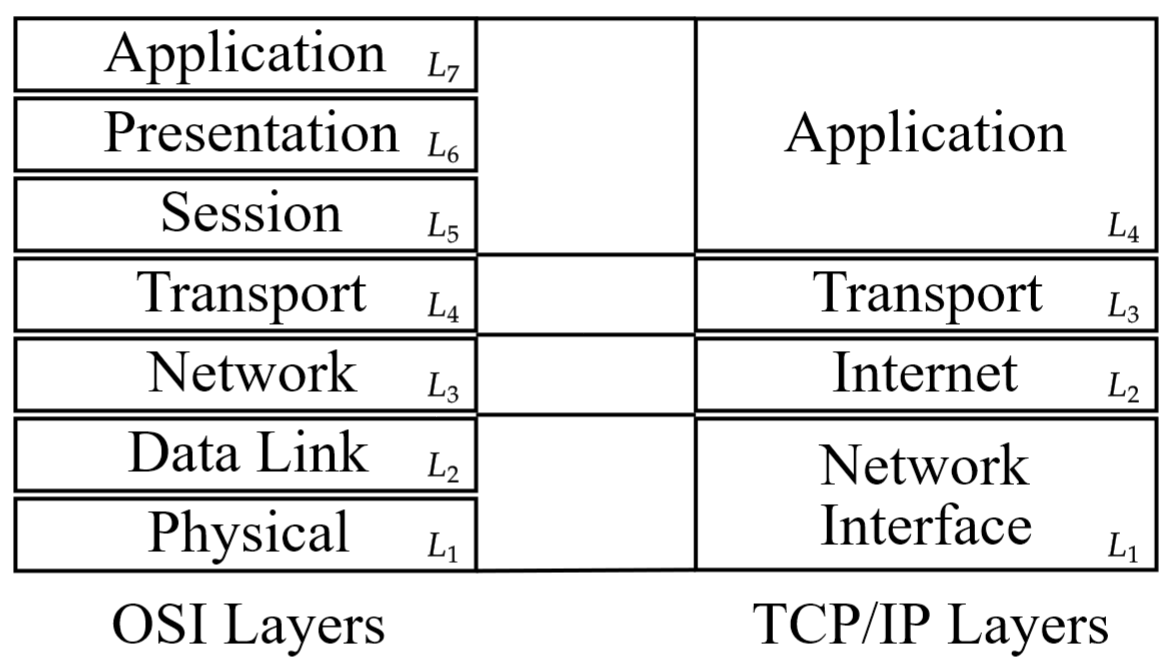
\includegraphics[width=0.7\textwidth]{Sections/network/osi_tcp.png}
    \caption{ISO vs TCP/IP Model}
    \label{fig:osi_tcpip}
\end{figure}

To illustrate two devices communicating over the internet, consider the diagram:

\section{Routing Networks}

\noindent
When IP addresses began


\begin{Def}[Routing]

    \textbf{Routing} is the process of selecting the best path across networks. 
    Data is segmented into packets, each with a destination address. 
    \textbf{Routers} are devices which forward this data through the network.

    Routers have a \textbf{routing table} which maps to other reachable networks. 
    When a packet arrives, the router checks against its routing table to find the best path.
    \hfill \cite{cloudflare_routing}
\end{Def}

\begin{Def}[Hop-by-Hop \& End-to-End Routing]

    \begin{itemize}
        \item  \textbf{Hop-by-Hop Routing}: When a packet of data is forwarded from one router to the next, a forward decision is called a \textbf{hop}.
        \item \textbf{End-to-End Routing}: The process of sending data from source to destination without intermediate hops.
    \end{itemize}
    \noindent
    It is often rare to see end-to-end routing in modern networks, as data is often forwarded through multiple routers. A target 
    destination may be unreachable from a given router.
    \hfill \cite{heimlicher_e2e_hbh}
\end{Def}

\newpage

\begin{Def}[Router Advertising]

    When routers inform each other of their existence and the networks they can reach \cite{narten_rfc4861}.
\end{Def}
\begin{Def}[Routing Protocols]
    
    \begin{itemize}
        \item \textbf{IP} (Internet Protocol): The primary protocol for routing data across the internet.
        \item \textbf{BGP} (Border Gateway Protocol): The protocol for routing data between \textbf{Autonomous Systems} (AS). 
        an AS is a collection of IP networks and routers under the control of a single entity (e.g., an \textbf{ISP} (Internet Service Provider)).
        These may only connect with each other if they have a mutual agreement. ASes identify themselves to 
        external networks using a unique \textbf{Autonomous System Number} (ASN).
        These are unique 16 bit numbers between 1-65534 or 32 bit numbers between 131072-4294967294 (e.g., \texttt{AS12345}) \cite{cloudflare_autonomous_system}.
        \item \textbf{OSPF} (Open Shortest Path First): A link-state routing protocol used within an AS. Link-state protocols are a set 
        of algorithms which determine the best path, based on the topology of a network graph \cite{kurose_link_state_routing}.
        It is also an \textbf{IGP} (Interior Gateway Protocol), meaning it operates within a single AS. It does so by sending out \textbf{LSAs} (Link State Advertisements) to other routers in the AS.
        Then routers in the system build a \textbf{LSADB} (Link State Advertisement Database) of the network topology. Then a shortest path algorithm is run to determine the best path to each network \cite{certbros_ospf_explained}.
        \item \textbf{RIP} (Routing Information Protocol): RIP employs hop count as a routing metric, with a maximum allowable hop count of 15 (network size limitation).
        It operates as an \textbf{IGP} within a single AS, periodically broadcasting the entire routing table to neighboring routers every 30 seconds,
        which can lead to slower convergence and higher bandwidth usage compared to other protocols. RIP is largely deprecated \cite{javatpoint_rip_protocol}.
    \end{itemize}
\end{Def}

\begin{Def}[IP Addressing]

    \textbf{IP addresses} are unique identifiers for devices on a network. 
    There are two versions of IP addresses, \textbf{IPv4} and \textbf{IPv6}.
    IPv4 A 32-bit address ($2^{32}$ addresses), employed since 1983, quickly exhausted all available addresses by the 2010s \cite{info12060246}.
    IPv6 is a 128-bit address ($2^{128}$ addresses), introduced in 1998 , in an attempt to address this shortage \cite{deering_ipv6_specification}\cite{ibm_ipv4_ipv6_formats}.
    For example,
    \begin{itemize}
        \item \textbf{IPv4}: a decimal octet ``$x.x.x.x$'': $x \in [0, 255]$ (e.g., \texttt{192.168.1.1}).
        \item \textbf{IPv6}: a hexadecimal segment ``$y:y:y:y:y:y:y:y$'': $y\in [0, FFFF]$ \\
         (e.g., \texttt{2001:0db8:85a3:0000:0000:8a2e:0370:7334}).
    \end{itemize}
\end{Def}

\newpage

\begin{Def}[Subnetting]

    Instead of a large monolith network of routers, networks can be divided into 
    smaller networks called \textbf{subnets}. I.e., Instead of passing data to every device on a network, routers forward data to a representative device on each subnet.
    \hfill \cite{cloudflare_subnet}
\end{Def}
\begin{Def}[Subnet Masking]

    A \textbf{subnet mask} defines which part of an IP address identifies the \textbf{network} and which part identifies the \textbf{host}.
\end{Def}
\begin{Def}[Classful Network]

    In the beginning, the first octet of an IPv4 address determined the network class---only allowing for 256 networks.
    The RFC\#791 published in 1981 introduced \textbf{Classful Networks} \cite{postel_internet_protocol}. 
    It uses the first three bits of the first octet's binary representation as a subnet mask to determine a class ranging from A-E.
    Th
\end{Def}

\begin{table}[h!]
    \centering
    \begin{tabular}{@{}p{.1cm}p{1.1cm}p{2cm}p{3cm}p{4cm}@{}}
    \toprule
    \textbf{Class} & \textbf{Binary Prefix} & \textbf{Range (Decimal)} & \textbf{Purpose} & \textbf{Details} \\ \midrule
    A              & \texttt{0xx}           & 1.0.0.0 to 126.0.0.0     & Unicast (large networks) & For large organizations; 8 bits for the network, 24 for hosts. \\
    B              & \texttt{10x}           & 128.0.0.0 to 191.255.0.0 & Unicast (medium networks) & For medium-sized networks; 16 bits for the network, 16 for hosts. \\
    C              & \texttt{110}           & 192.0.0.0 to 223.255.255.0 & Unicast (small networks) & For small networks; 24 bits for the network, 8 for hosts. \\
    D              & \texttt{1110}          & 224.0.0.0 to 239.255.255.255 & Multicast & Reserved for multicast addressing; not for general use. \\
    E              & \texttt{1111}          & 240.0.0.0 to 255.255.255.255 & Experimental and future use & Reserved for research and development; not assigned for standard use. \\ \bottomrule
    \end{tabular}
    \caption{Overview of IPv4 Address Classes}
    \label{tab:ipv4_classes}
\end{table}






\newpage 

\noindent 

\begin{Def}[Fixed Length Subnet Masking (FLSM)]

    \textbf{Fixed Length Subnet Masking} (FLSM) is a technique which divides a network into equal-sized subnets. This
    may lead to inefficient use of IP addresses.
    \hfill \cite{awati_vlsm}
\end{Def}
\begin{Def}[Variable Length Subnet Masking (VLSM)]

    \textbf{Variable Length Subnet Masking} (VLSM) is a technique which allows for the creation of subnets with different sizes. 
    As some ASes may require more IP addresses than others, VLSM allows for more efficient use of IP addresses.
    \hfill \cite{awati_vlsm}
\end{Def}
\noindent

\begin{Def}[Classless Inter-Domain Routing (CIDR)]

    \textbf{Classless Inter-Domain Routing} (CIDR), introduced in 1993 through RFC\#1518 and RFC\#1519 to address IPv4 exhaustion.
    \textbf{CIDR replaced classful subnetting} with VLSM.

    \noindent
    CIDR notation is written as \underline{\texttt{IP Address/Prefix Length} (e.g., \texttt{192.168.1.0/24})}, where:
    \begin{itemize}
        \item \texttt{IP Address}: Represents the starting address of the network.
        \item \texttt{Prefix Length}: The number of bits used for the \textbf{network portion} of the address.\\
    \end{itemize}

    \vspace{-1em}
    \noindent
    For example:\\

        \vspace{-1em}
        \begin{center}
            \large
            \texttt{255.0.0.0\textbf{/8}}; \hspace{.2em} \texttt{255.255.0.0\textbf{/16}}; \hspace{.2em} \texttt{255.255.255.0\textbf{/24}}; \hspace{.2em} \texttt{255.255.255.192\textbf{/26}};
            \normalsize
        \end{center}
    \hfill \cite{fuller_cidr_rfc1519}
\end{Def}

\begin{Def}[Route Aggregation]

    CIDR introduced \textbf{Route Aggregation} also known as \textbf{Supernetting}, or \textbf{Route Summarization}, is the process of combining multiple routes into a single route advertisement.
    \textbf{Example}:
    Consider an organization assigned the following contiguous IP address blocks:
    \begin{center}
        \texttt{192.168.\textbf{1}.0/24}; \quad \texttt{192.168.\textbf{2}.0/24}; \quad \texttt{192.168.\textbf{3}.0/24}; \quad \texttt{192.168.\textbf{4}.0/24};
    \end{center}
    Each block holding 256 IP addresses with a subnet mask of 255.255.255.0, requiring four routing table entries. 
    However, these networks share a common prefix: the first 22 bits (\texttt{192.168.0.0/22}), which aggregates to: \texttt{\textbf{192.168.0.0/22}} \cite{fuller_cidr_rfc1519}.

\end{Def}
\newpage
\begin{Def}[IP Address Components]
    
        \item \textbf{Network Address}:
        \begin{itemize}
            \item Identifies the specific network segment to which a device is connected.
            \item Determined by setting all bits in the host portion to 0.
            \item Example: For the IP address \texttt{192.168.1.10} with a subnet mask of \texttt{255.255.255.0} (/24), the network address is \texttt{192.168.1.0}.
        \end{itemize}

        \item \textbf{Host Address}:
        \begin{itemize}
            \item Uniquely identifies a device within a network segment.
            \item The bits in the IP address designated for hosts, specified by the subnet mask.
            \item Example: In the IP address \texttt{192.168.1.10} with a /24 subnet mask, the host portion is the last octet (10).
        \end{itemize}

        \item \textbf{Broadcast Address}:
        \begin{itemize}
            \item Used to communicate with all devices on a specific network segment simultaneously.
            \item Determined by setting all bits in the host portion to 1.
            \item Example: For the network \texttt{192.168.1.0/24}, the broadcast address is \texttt{192.168.1.255}.
        \end{itemize}
      

    \hfill \cite{sunshine_rfc919} \cite{postel_rfc922} \cite{manning_rfc1878}

\end{Def}
\noindent
Consider the IP address \texttt{192.168.2.12/26} and its binary \texttt{11000000.10101000.00000010.00001100}:

\vspace{-1em}
\begin{figure}[h!]
    \hspace{2em}
    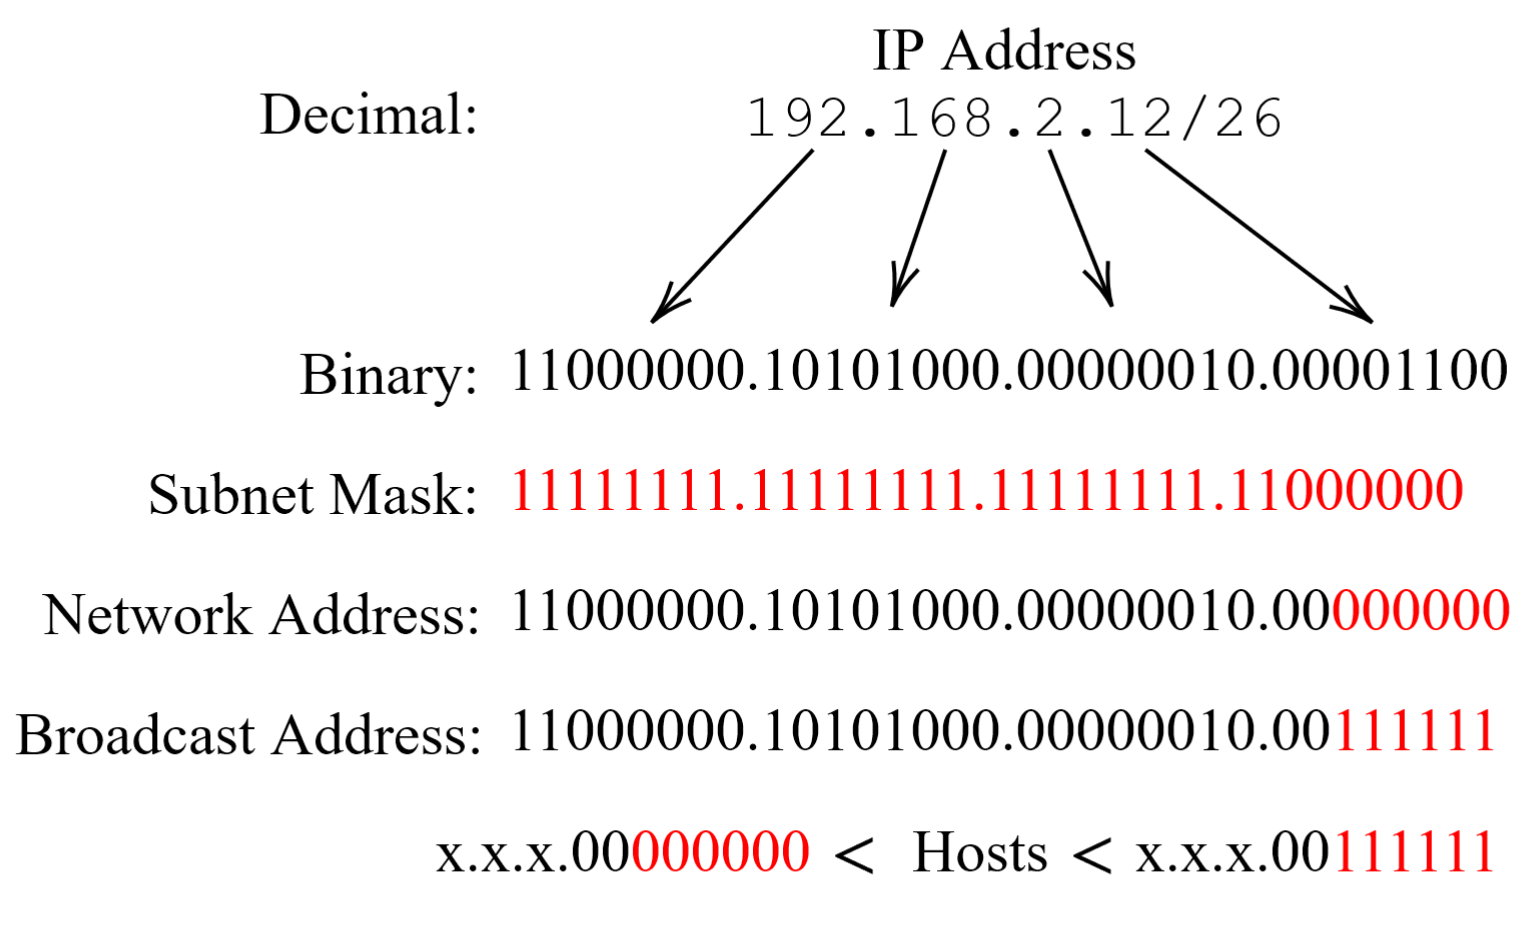
\includegraphics[width=0.7\textwidth]{Sections/network/ip_address.png}
    \caption{Binary Subnetting: Red indicating parts of the IP address identified for each component.}
    \label{fig:subnetting}
\end{figure}
\noindent
\begin{Def}[Common Types of Area Networks (ANs)]

    \textbf{PAN (Personal Area Network)}: A network for personal devices, such as smartphones, smartwatches, or earbuds, with a short range (typically a few meters) using technologies like Bluetooth or infrared.\\

    \noindent
    \textbf{LAN (Local Area Network)}: Connects devices within a small area, such as a home, office, or school, enabling high-speed communication and resource sharing.\\

    \noindent
    \textbf{WLAN (Wireless Local Area Network)}: A wireless version of LAN that uses Wi-Fi to connect devices within a localized area like a home or office.\\

    \noindent
    \textbf{CAN (Campus Area Network)}: A network that connects multiple LANs across a limited geographical area, such as a university campus or corporate facility, for resource sharing and communication.\\

    \noindent
    \textbf{MAN (Metropolitan Area Network)}: Covers a larger area than a LAN, typically a city or metropolitan region, connecting multiple LANs or CANs via high-speed infrastructure like fiber optics.\\

    \noindent
    \textbf{WAN (Wide Area Network)}: Connects LANs, MANs, or other networks over large geographical areas, such as countries or continents. The internet is the largest WAN example.\\

    \noindent
    \textbf{SAN (Storage Area Network)}: A high-speed network that provides access to storage devices for data centers, ensuring fast and reliable storage management.\\

    \noindent
    \textbf{EPN (Enterprise Private Network)}: A private network created by organizations to connect their various locations securely, often including VPNs for remote access.\\

    \noindent
    \textbf{VPN (Virtual Private Network)}: Creates a secure, encrypted connection over public networks, like the internet, to allow users to access private networks remotely.\\

    \noindent
    \textbf{HAN (Home Area Network)}: A network within a home environment, connecting personal devices like computers, printers, and smart home gadgets.\\

    \noindent
    \textbf{GAN (Global Area Network)}: A large-scale network that connects multiple WANs and supports worldwide communication, with the internet as its most prominent example.

    \hfill \cite{petryschuk_types_of_networks}
\end{Def}

\newpage 

\begin{Example}[Subnetting a Network via VLSM]


Consider the FLSM below, which all have 62 hosts per network:
\[
\begin{array}{|c|c|c|}
\hline
\textbf{Network Address} & \textbf{Hosts} & \textbf{Broadcast Address} \\ \hline
192.168.100.0 & .1 - .62 & .63 \\ \hline
192.168.100.64 & .65 - .126 & .127 \\ \hline
192.168.100.128 & .129 - .190 & .191 \\ \hline
192.168.100.192 & .193 - .254 & .255 \\ \hline
\end{array}
\]
\noindent
Below illustrates this network, where a router of base address \texttt{192.168.1.0/24},
connects four LANs:\\

\hspace{4em}
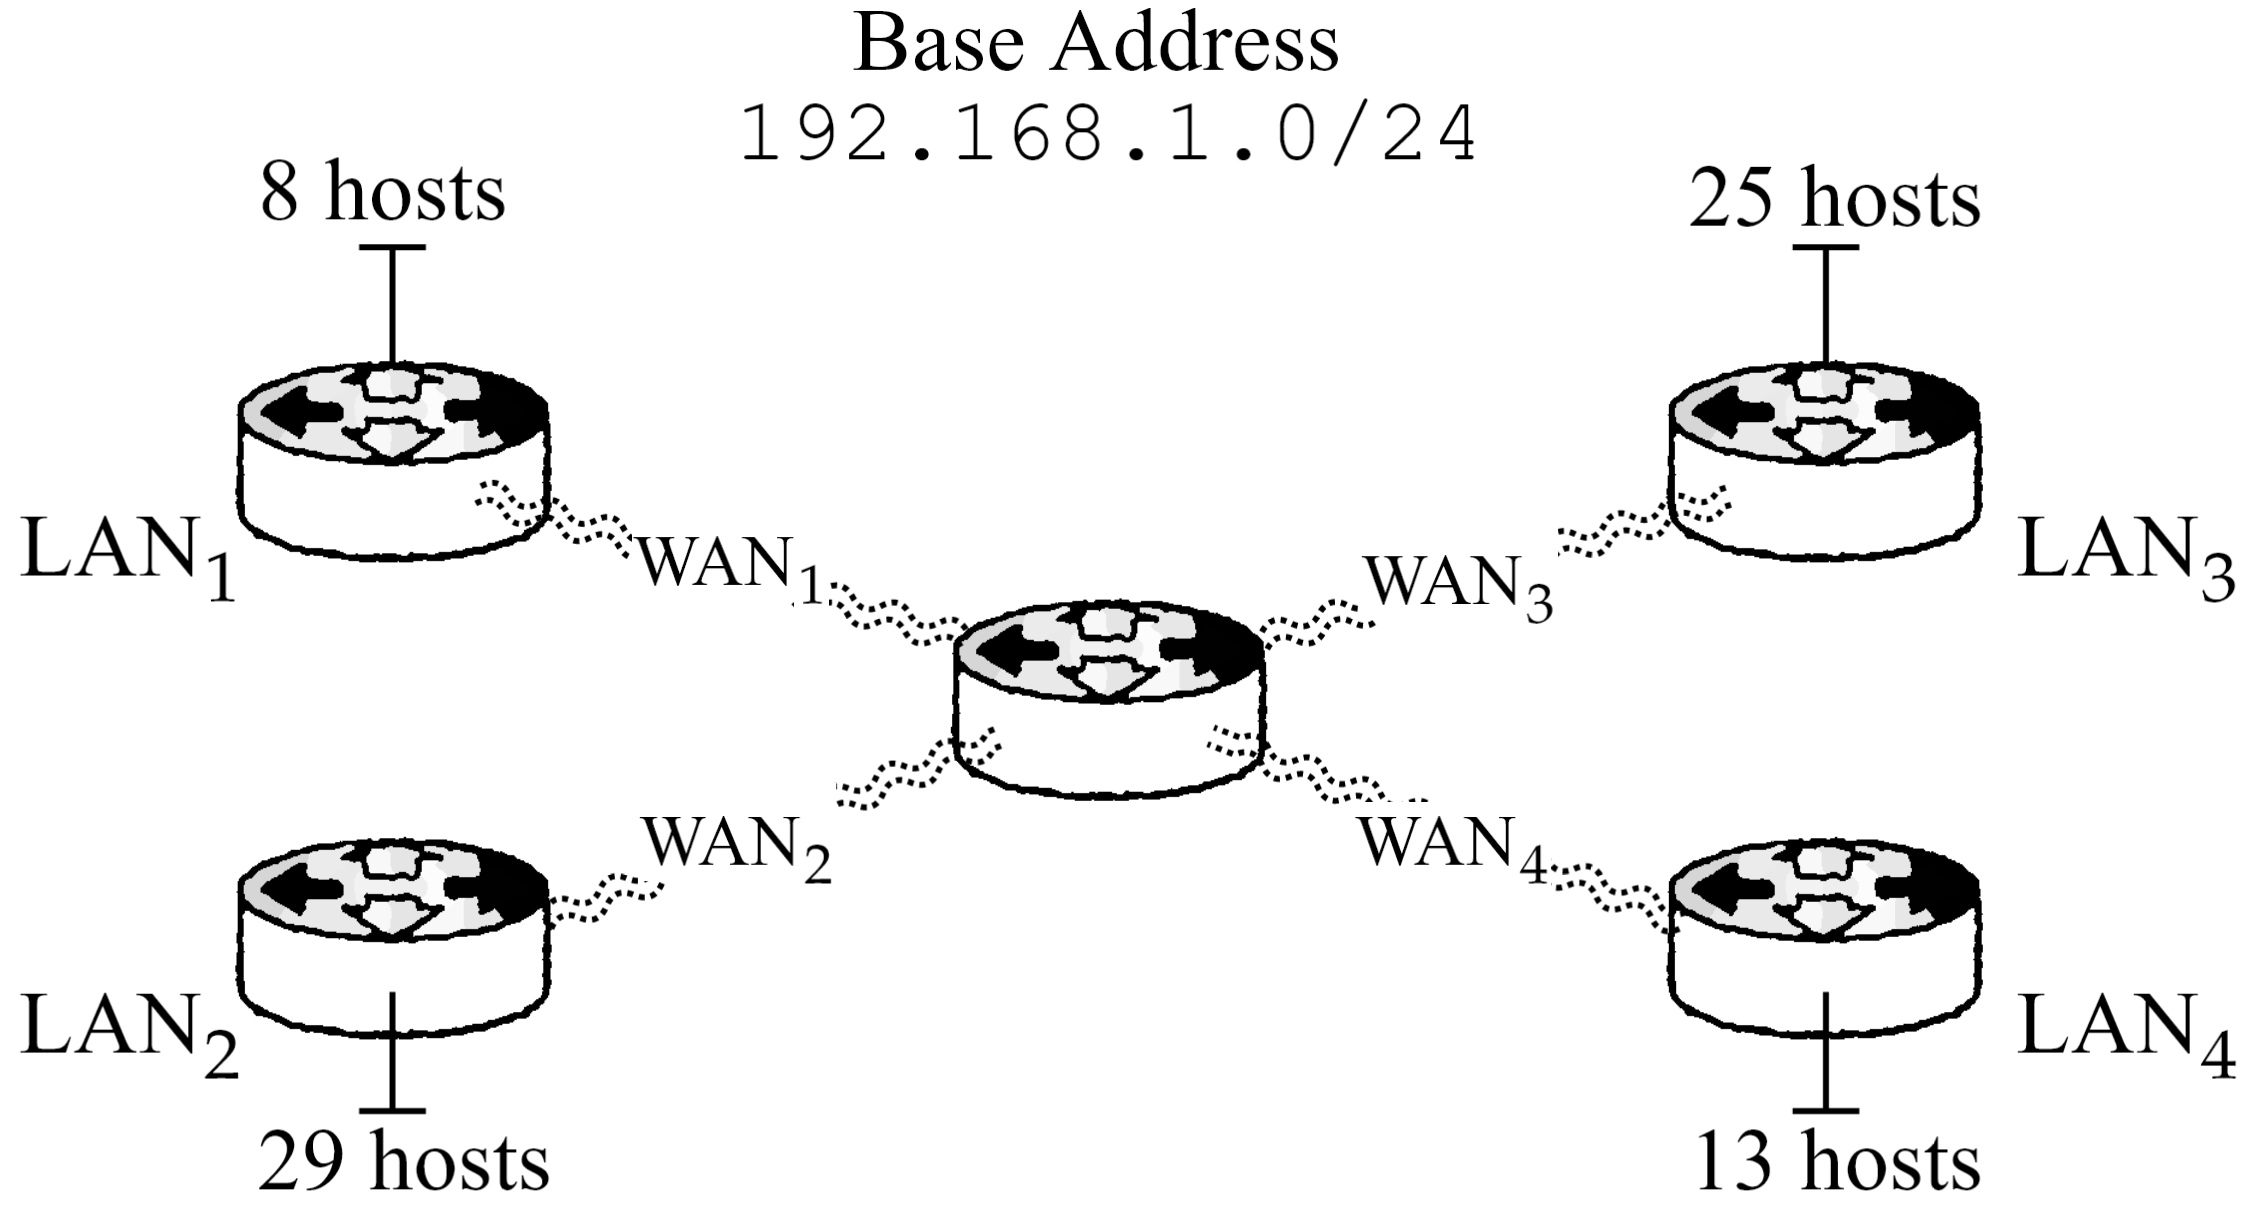
\includegraphics[width=0.7\textwidth]{Sections/network/subnetting.png}\\

\noindent
\textbf{Subnetting:} Process each LAN from largest to smallest, Select the nearest block size, identify the network, host, and broadcast addresses.
Since there is a subnet mask of /24, blocks $[128, 64, 32, 16, 8, 4, 2, 1]$ are available. This is the case as 
$2^8 = 256$. If a LAN has 129 hosts, that LAN will occupy all 254 addresses (as x.x.x.0 and x.x.x.255 are reserved).\\
\begin{enumerate}
    \item \textbf{LAN$_2$}: 29 hosts $\Rightarrow$ Block size 32. Network: \texttt{x.0}, Broadcast: \texttt{x.31}, Hosts: \texttt{x.1-x.30}.
    \item \textbf{LAN$_3$}: 25 hosts $\Rightarrow$ Block size 32. Network: \texttt{x.32}, Broadcast: \texttt{x.63}, Hosts: \texttt{x.33-x.62}.
    \item \textbf{LAN$_4$}: 13 hosts $\Rightarrow$ Block size 16. Network: \texttt{x.64}, Broadcast: \texttt{x.79}, Hosts: \texttt{x.65-x.78}.
    \item \textbf{LAN$_1$}: 8 hosts $\Rightarrow$ Block size 16. Network: \texttt{x.80}, Broadcast: \texttt{x.95}, Hosts: \texttt{x.81-x.94}.
\end{enumerate}

\noindent
8 hosts need occupy 16, as a block size of 8 only has 6 usable addresses. The computed subnet now only occupies addresses 
\texttt{x.0-x.95}, leaving room for additional LANs \cite{eastcharmer_vlsm_subnetting}. 

\end{Example}
    



